% ====================================================================
%%- Arvhivo de ejemplo para la clase ThesisUTPL -%%
% ====================================================================
%  *Texto de ejemplo para el Anexo 1*
% ====================================================================
% Creado por: Francisco Alberto Sandoval Noreña
% e-mail: fasandoval@utpl.edu.ec
%
% Version 1.1.0
% Date: 07/11/2019
%
% Fecha de creación: 11 de noviembre de 2018
% Version: 0.1
% ====================================================================
%
%%- Inicio del Texto -%% ---------------------------------------------
\chapter{Acelerador de Partículas del Laboratorio S.T.A.R. y sus Impactos en la Fuerza de Velocidad}

\Blindtext

Ejemplo de figura en Anexo (ver \autoref{fig:utplcruzAnexo}). 

\begin{figure}[h!]
	\centering
	\captionsetup{width=0.7\textwidth}
	\caption{Campus UTPL (Anexo) \vspace{-5pt}}
	\label{fig:utplcruzAnexo}
	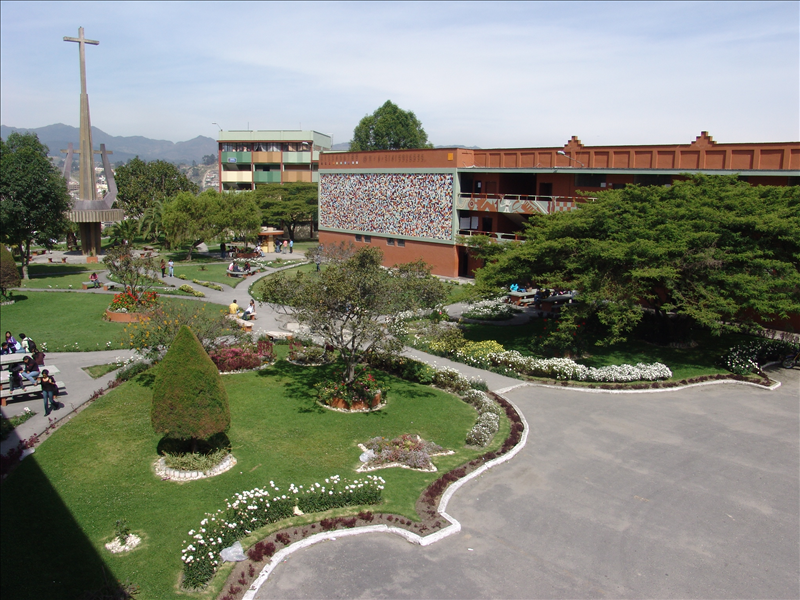
\includegraphics[width=0.7\linewidth]{FIGURES/UTPL_cruz}
	\NotaCaptionUTPL{Fotografía de la Universidad Técnica Particular de Loja (UTPL) \autocite{utpl2008campus}}
\end{figure}

Ejemplo de tabla en Anexo (ver \autoref{tb:EjemploAnexo}).

\begin{table}[h!]
	\centering
	\captionsetup{width=0.44\textwidth}
	\caption{Ejemplo de tabla en Anexo}
	\label{tb:EjemploAnexo}
	\begin{tabular}{|l|l|l|}
		\hline
		\textbf{Columna 1} & \textbf{Columna 2} & \textbf{Columna 3} \\ \hline
		ítem 1             & ítem 2             & ítem 3             \\ \hline
		ítem 4             & ítem 5             & ítem 6             \\ \hline
		ítem 7             & ítem 8             & ítem 9             \\ \hline
	\end{tabular}
	\NotaCaptionUTPL{}		
\end{table}


